\documentclass[english]{tktltiki}
\usepackage[pdftex]{graphicx}
\usepackage{subfigure}
\usepackage{url}
\usepackage{enumerate}
\begin{document}
%\doublespacing
%\singlespacing
\onehalfspacing

\title{Advanced course in Machine Learning - Week 1}
\author{P�ter Ivanics}
\date{\today}

\maketitle

Time spent on this set of exercises: 10 hours

\section{Background information}

\begin{enumerate}[a)]
	\item I have taken only the "Introduction to Machine Learning" course during the Autumn 2016 semester at University of Helsinki. I have not taken any courses in this field at the University of Helsinki otherwise. Nevertheless, during my first Bachelor degree I have taken a course in Probability and Statistics at �buda University in 2011. 
	\item I have some knowledge in statistics and I am familiar with the basic concepts, but advanced topics are fairly unknown to me as it turned out during the course last semester - I would say around 3
	\item For similar reasons, around 3
	\item The reason why I have taken this course is that I greatly enjoyed the preliminary course mentioned above. Additionally, I have started studying on this master programme to enhance my knowledge in this topic and I believe this is a direction to which I should specialize and dig deeper into. 
	\item I would like to learn about the application fields of machine learning and understand the capabilities. I would like to know what kind of open APIs exist in case I would have to use some classifier for my work or projects. Additionally, I am more than happy to implement some "common" algorithms myself and see how they perform on different datasets and distributions. The best outcome from this course for me personally would be the knowledge, what I can apply straight to my work as a software developer and come up with a suggestion how Machine Learning could be utilized at the company I am working for. I would be happy to solve more computer-based tasks over pen and paper exercises. 
\end{enumerate}

\section{Expectations}
\begin{center}
	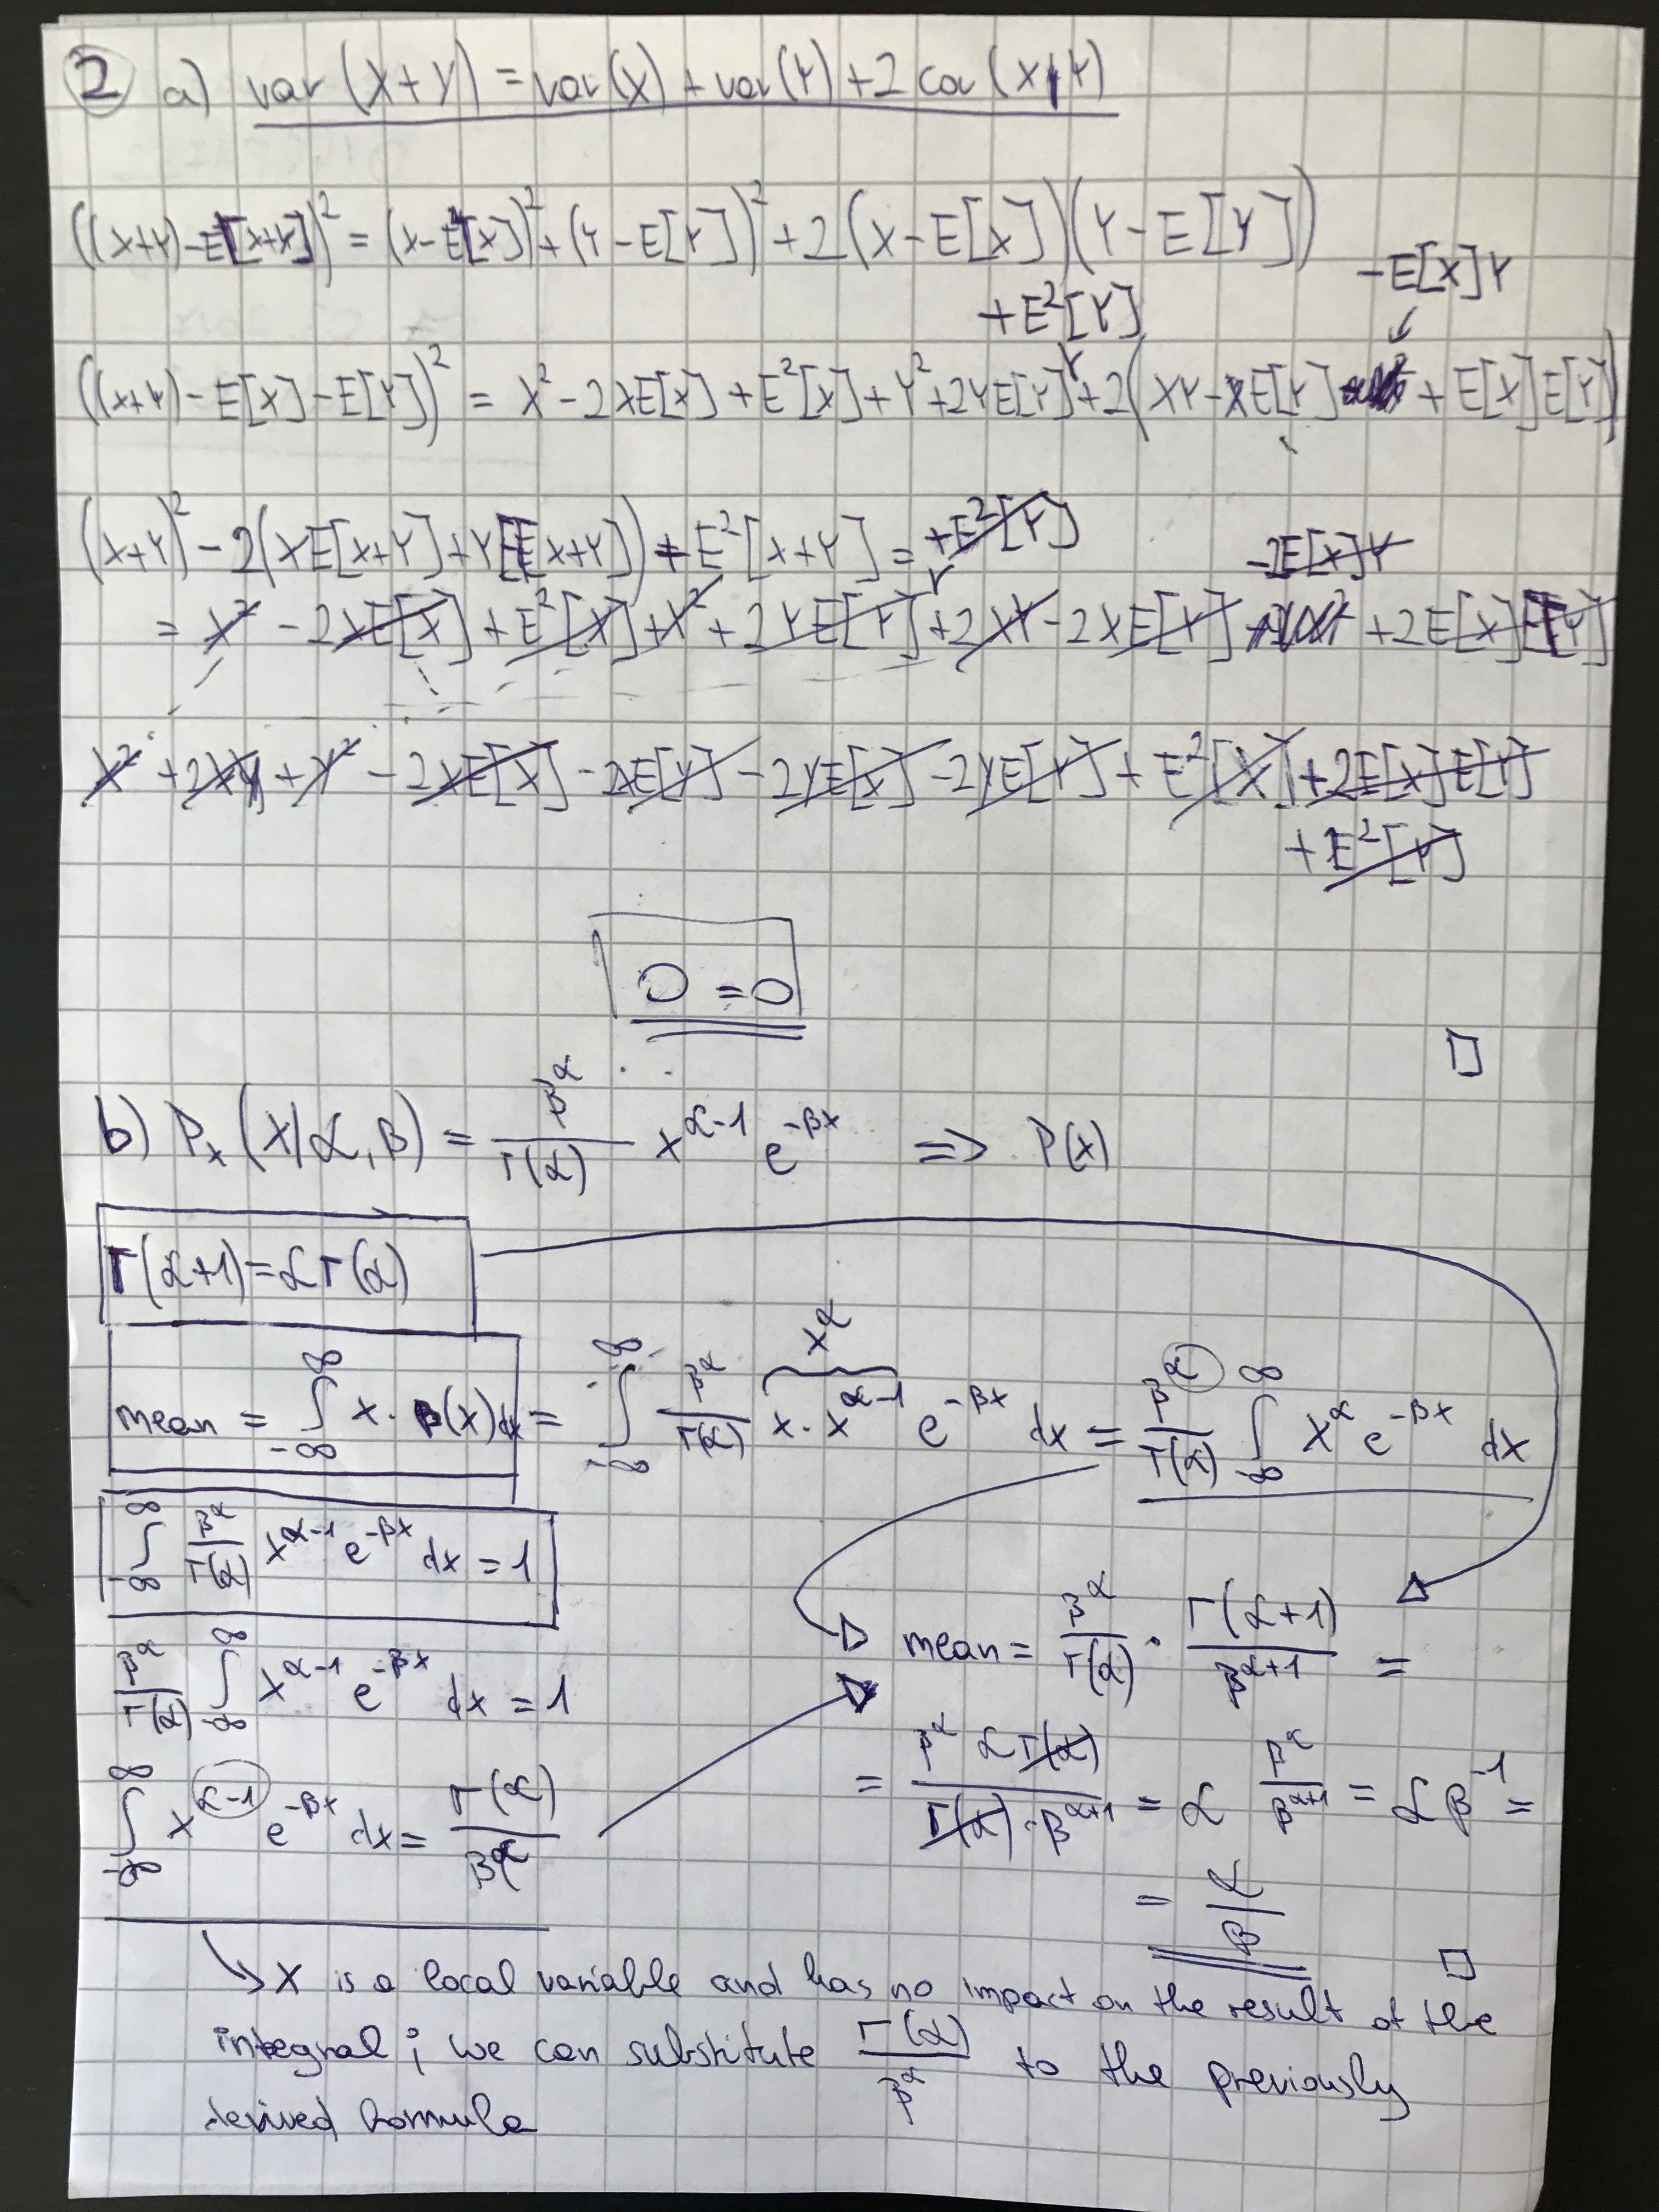
\includegraphics[width=1\textwidth]{images/IMG_0074.jpg}
\end{center}

\section{Eigen-value decomposition}
\begin{enumerate}
	\item After loading the dataset we can see that the number of observations (rows) in the dataset is N=200 and the number of dimensions (columns) is D=5. 
	\item The Eigenvalues of the covariance matrix \textbf{X} are, as follows (see $Eigen-value\_decomposition.r$ for implementation): 
	\begin{center}
		$[2.012649572, 0.222861976, 0.142902106, 0.010428670, 0.009259117]$
	\end{center}
	\item After reducing the data to the $L=2$ first eigenvectors, it is reduced to two dimensions. A plot of this dataset is displayed on the figure below. As we can see, after performing the dimension reduction, the data has only two dimensions (X and Y). 
	
	\begin{center}
		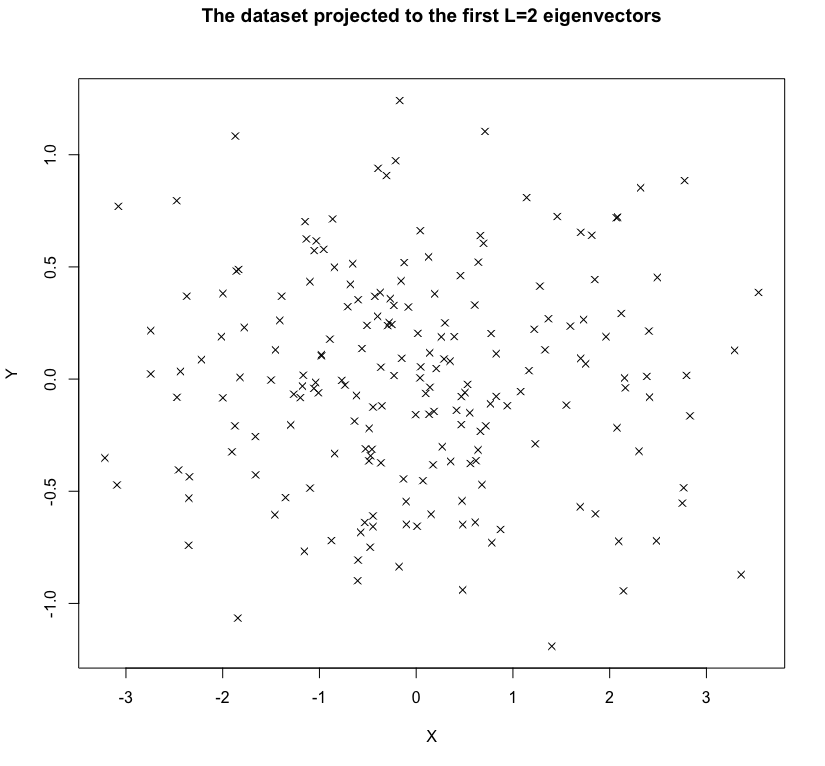
\includegraphics[width=0.75\textwidth]{images/first_two_eigenvectors.png}
	\end{center}
	\item The reconstruction error for L=2,3,4,5 is displayed on the figure below. We can see that linearly with the number of reduced dimensions, the reconstruction error increases. For L=5, the reconstruction error is therefore 0. We can also observe that the reconstruction error dramatically increases when we would like to reduce the data to 2 dimensions only, while for 3 and 4 dimensions it remains considerably low. 
	\begin{center}
		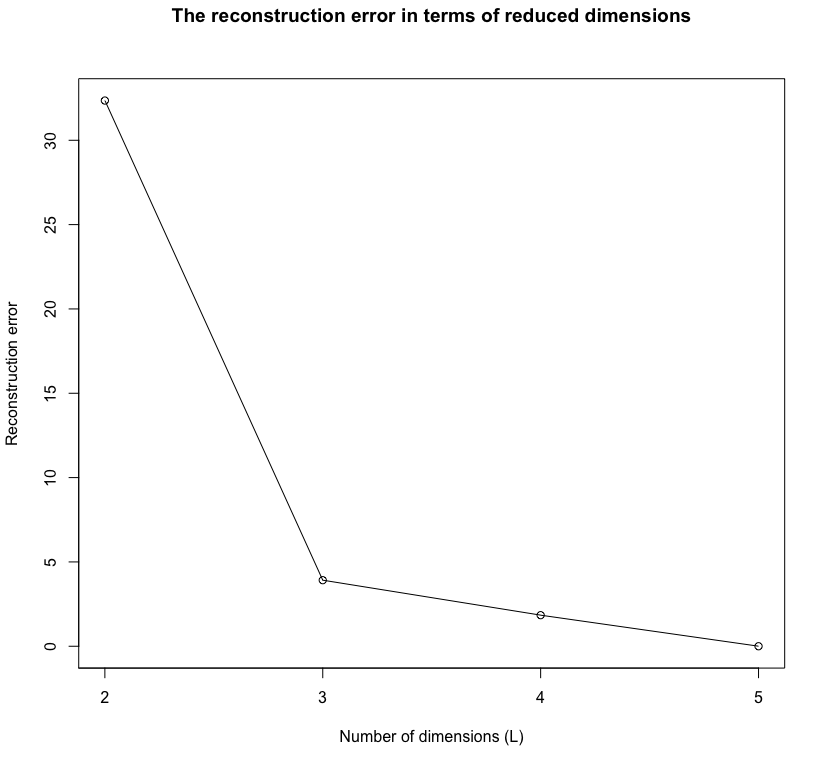
\includegraphics[width=0.75\textwidth]{images/reconstruction_error.png}
	\end{center}
\end{enumerate}
\section{Derivatives, gradients and all that}
\begin{enumerate}[a)]
	\item First, we find the derivate function of the sigmoid function, as follows: 

	\begin{center}
		$s(z) = \frac{1}{1 + e^{-z}}$ \\
	\end{center}

	Let $u = e^x + 1$ and $\frac{d}{d u} \frac{1}{u} = - \frac{1}{u ^ 2}$. Using the chain rule of derivation, we can see that

	\begin{center}
		$s'(z)dz = - \frac{\frac{d}{dz}(1+ e^z)}{(e^z + 1)^2} = - \frac{e^z}{(e^z + 1)^2}$
	\end{center}

	Next, we derive the given logarithmic loss function to see that $\frac{dL}{d\theta_i} = x_i(s(\theta^Tx) - y)$

	\begin{center}
		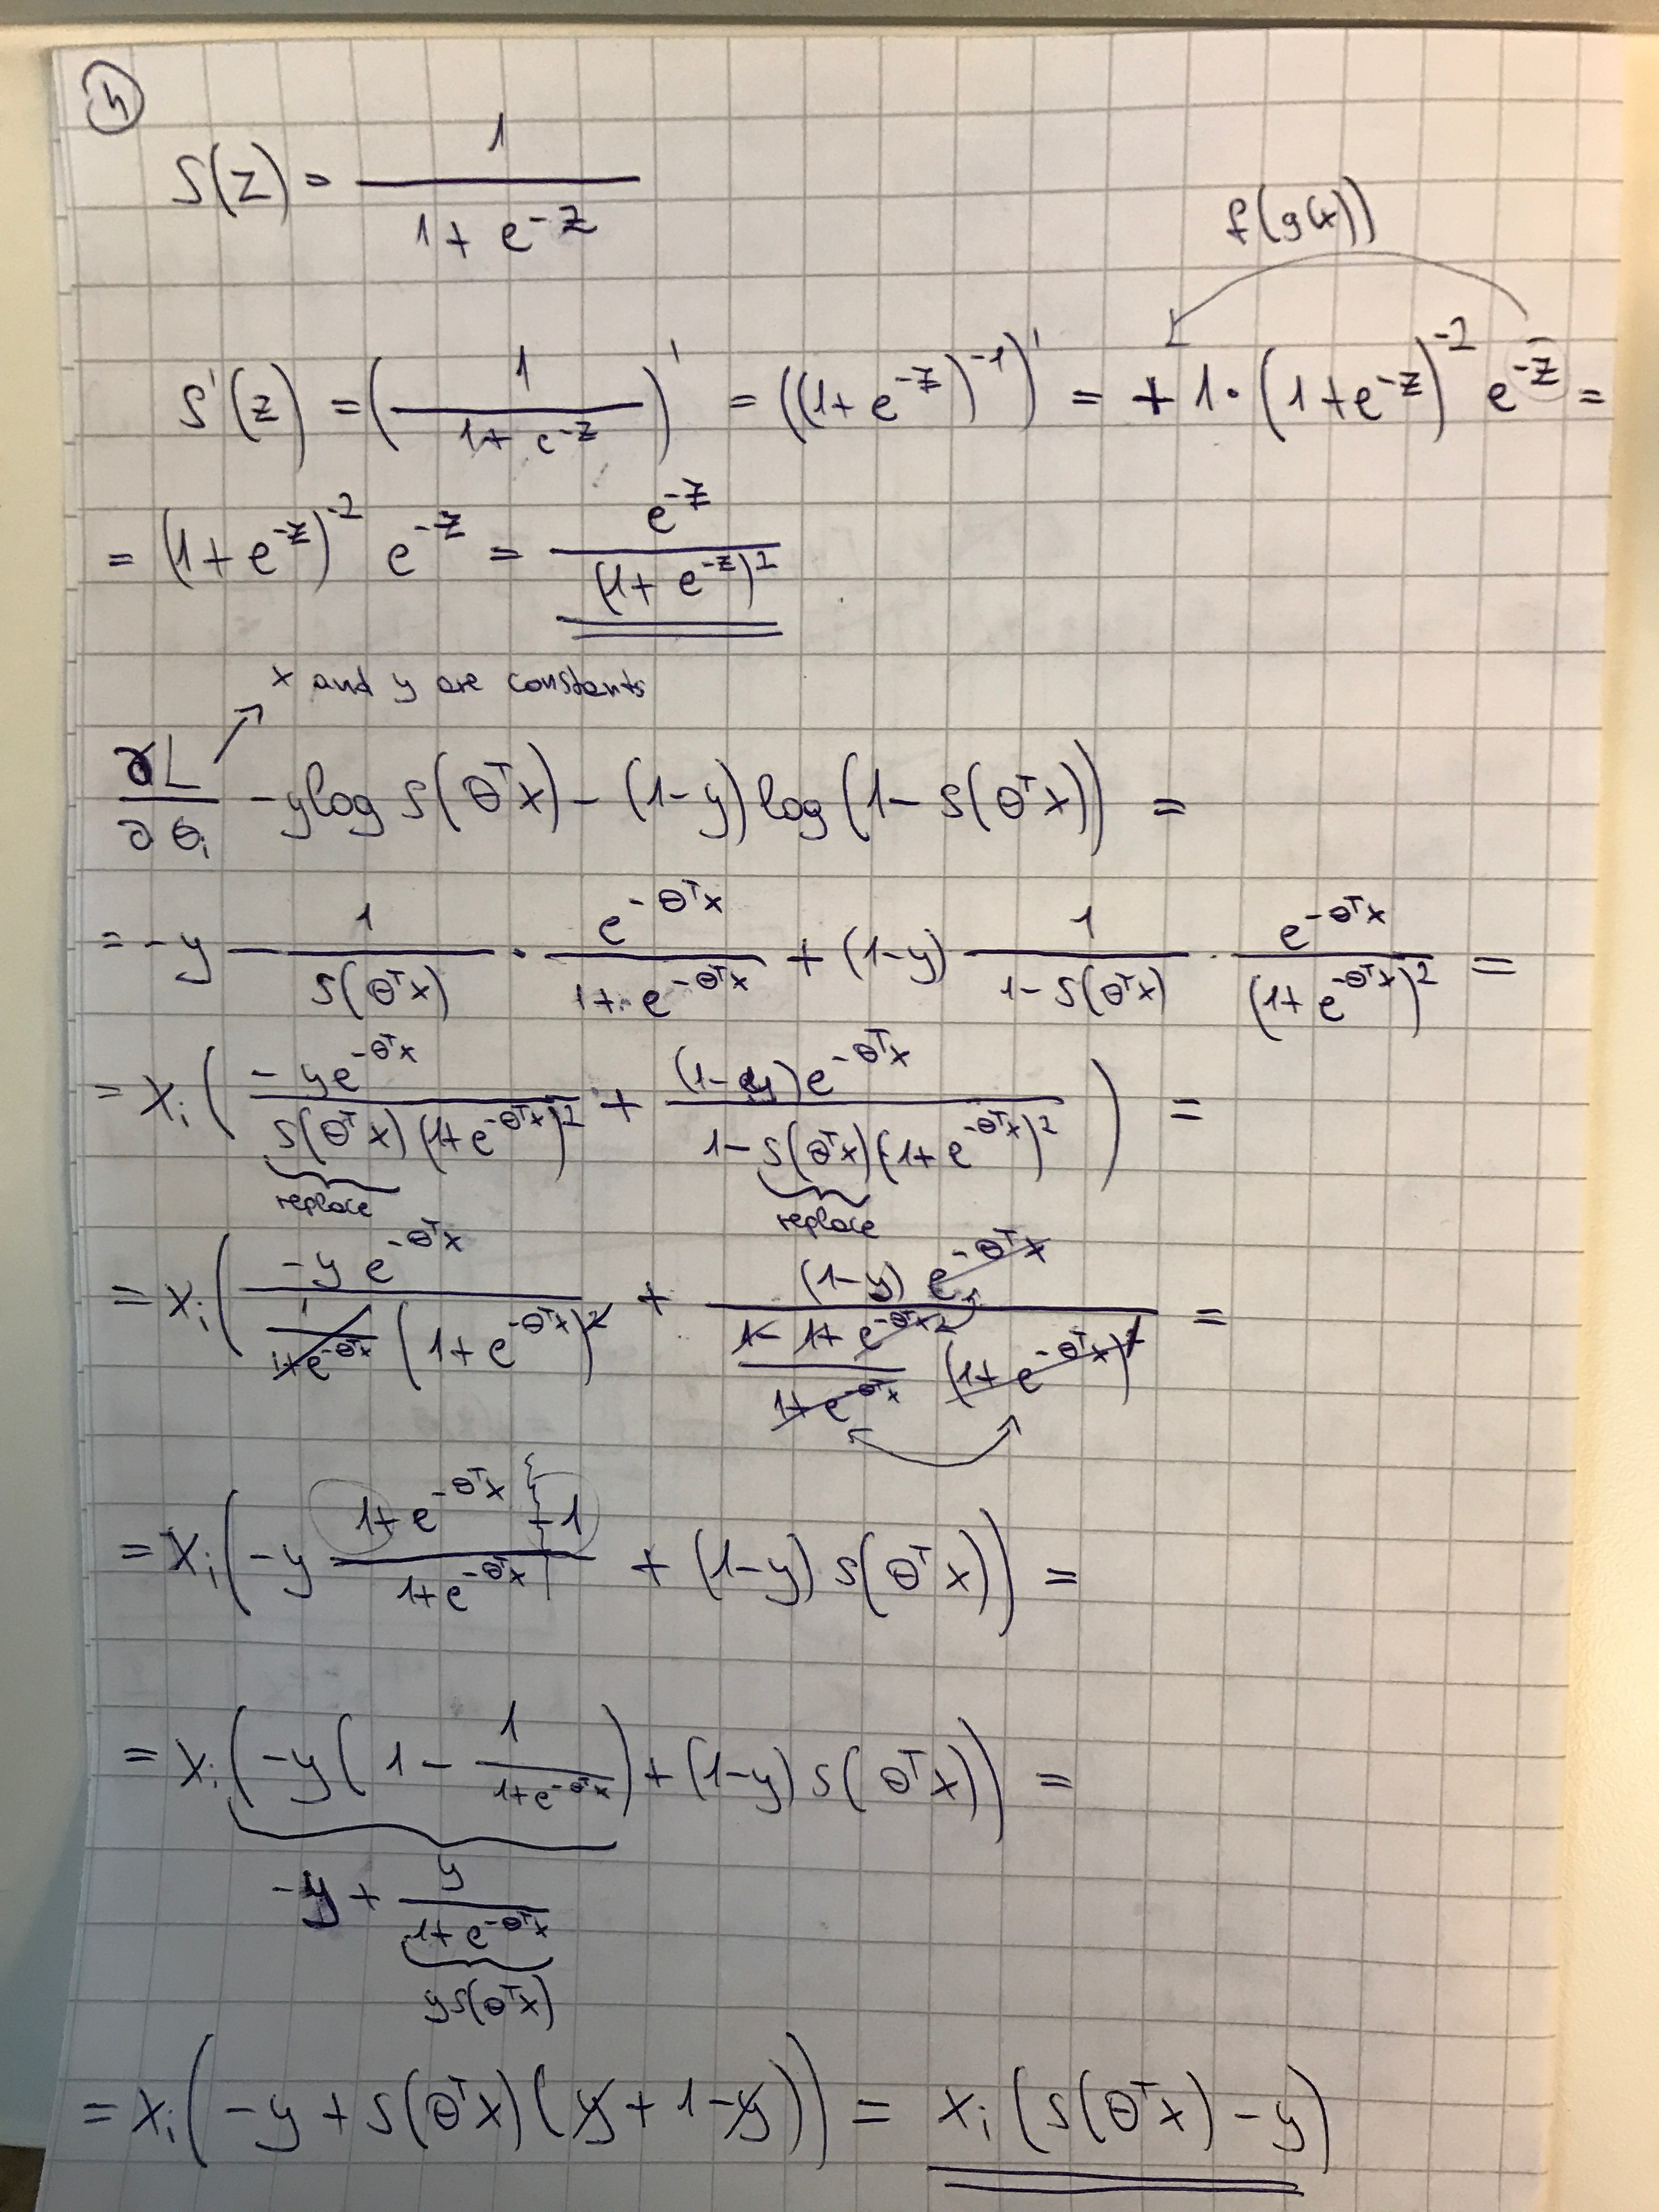
\includegraphics[width=1\textwidth]{images/IMG_0144.jpg}
	\end{center}
	\item Similarly to the previous item, we can derive the second derivate from the result, as follows.
	
	\begin{eqnarray*}
		\frac{d}{d\theta}(x(s(\theta ^ Tx) - y))' = \\
		= x * \frac{d}{d\theta}((s(\theta ^ T x) - y))' = \\
		= x(\frac{e^{-\theta ^ T x}}{(1 + e ^{- \theta ^ T x})^2 } * x)
	\end{eqnarray*}
	\item We can use this to calculate the gradient using the result item a) with the given values (see $gradient.R$ for implementation). This yields in 

	\begin{center}
		$\nabla L ((x, y), \theta) = [0.2689414, -0.5378828]$
	\end{center}
	
	\item Similarly, the second derivatives by $\theta$ can be obtained and used to calculate the Hessian matrix: 
	
	\begin{center}
		$H (L ((x, y), \theta)) = $
		
		\begin{tabular}{cc}
				0.1966119 & -0.3932239 \\
			   -0.3932239 &  0.7864477
		\end{tabular}
	\end{center}
\end{enumerate}

\lastpage

\end{document}